\appendix
\chapter{Appendices}
\section{Appendix A}
\subsection{Use Case Diagram example (Online Shopping System)}
\begin{figure}[H] % Use 'H' to place the figure exactly here
    \centering
    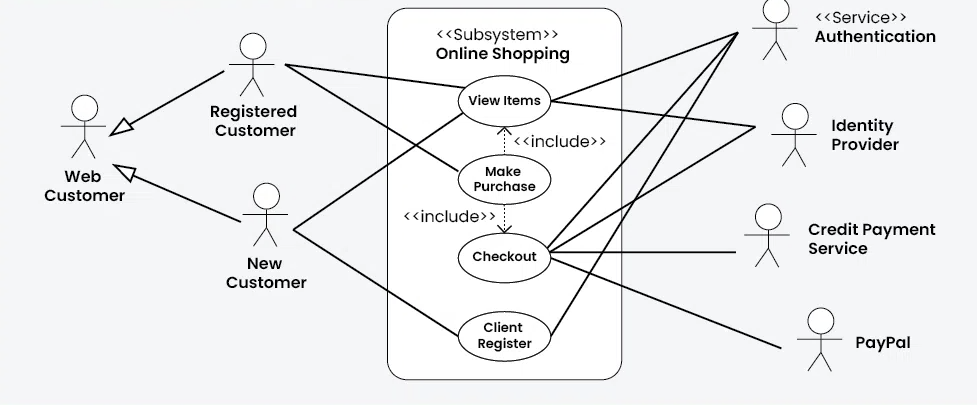
\includegraphics[width=\textwidth]{images/usecaseexample.png}
    \caption{Use Case Diagram for the Online Shopping System}
    \label{fig:usecase1}
\end{figure}

\subsection{Detail Use Case Example}
\begin{figure}[H] % Use 'H' to place the figure exactly here
    \centering
    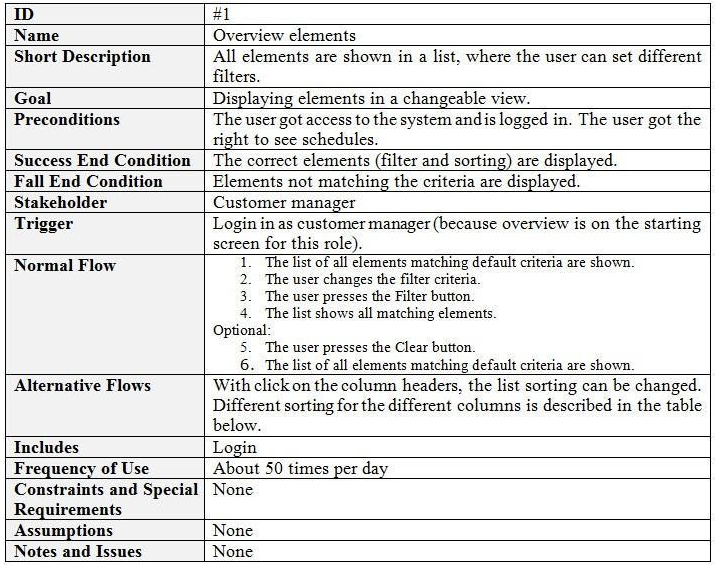
\includegraphics[width=\textwidth]{images/detailusecase.png}
    \caption{Detail Use Case Example}
    \label{fig:usecase2}
\end{figure}

\subsection{Event-Response Table for a Highway Intersection}
\begin{figure}[H] % Use 'H' to place the figure exactly here
    \centering
    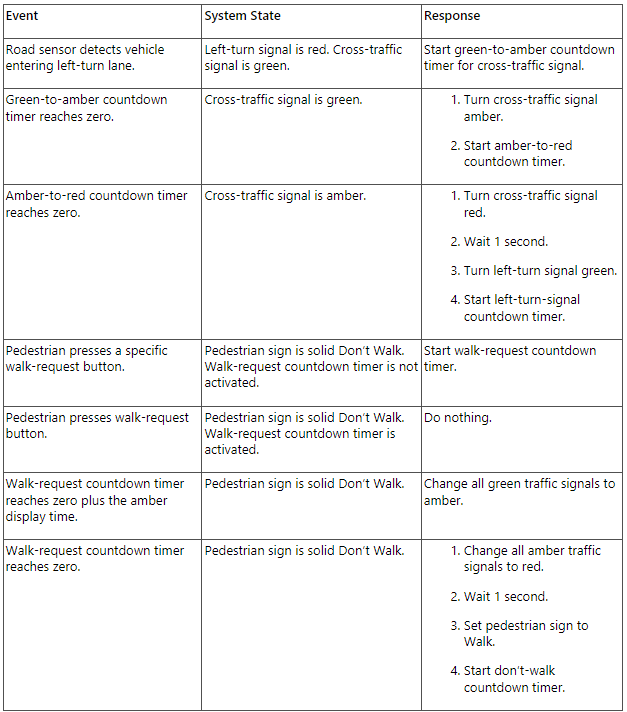
\includegraphics[width=\textwidth]{images/eventresponsetable.png}
    \caption{Example of Event Response Table}
    \label{fig:usecase3}
\end{figure}

\subsection{Story Board Example For Android App}
\begin{figure}[H] % Use 'H' to place the figure exactly here
    \centering
    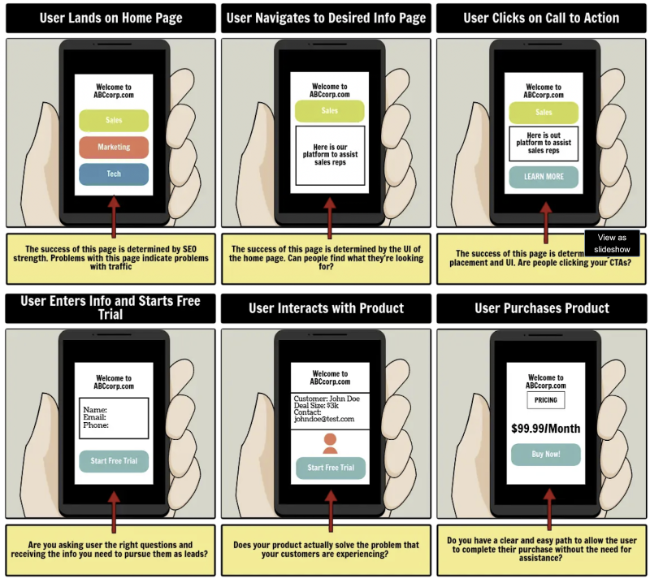
\includegraphics[width=\textwidth]{images/storyboard.png}
    \caption{Example of Story Board}
    \label{fig:usecase3}
\end{figure}

\section{Appendix B}

\subsection{Domain Model Example For Online Shopping}
\begin{figure}[H] % Use 'H' to place the figure exactly here
    \centering
    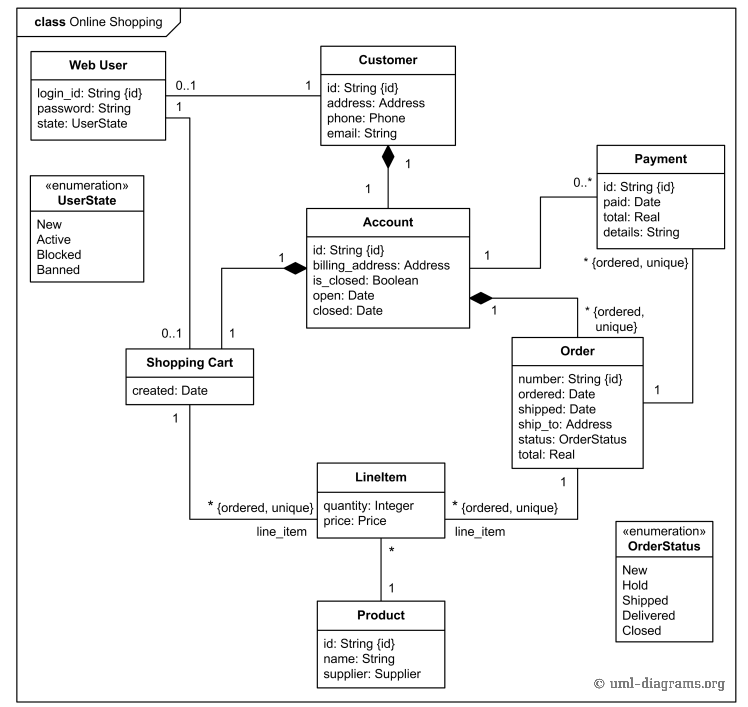
\includegraphics[width=\textwidth]{images/domainmodel.png}
    \caption{Domain Model Example For Online Shopping Application}
    \label{fig:usecase3}
\end{figure}


\section{Appendix C}

\subsection{Box And Line Example For Online Shopping}
\begin{figure}[H] % Use 'H' to place the figure exactly here
    \centering
    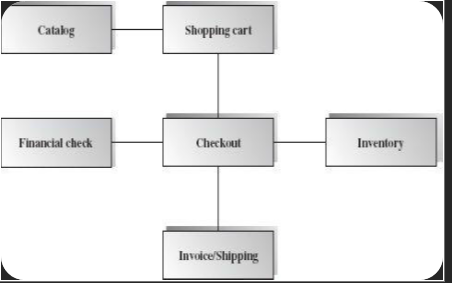
\includegraphics[width=\textwidth]{images/boxandline.png}
    \caption{Box and Line Diagram For Online Shopping Application}
    \label{fig:usecase3}
\end{figure}

\subsection{Architecture Pattern Example For Online Shopping}
\begin{figure}[H] % Use 'H' to place the figure exactly here
    \centering
    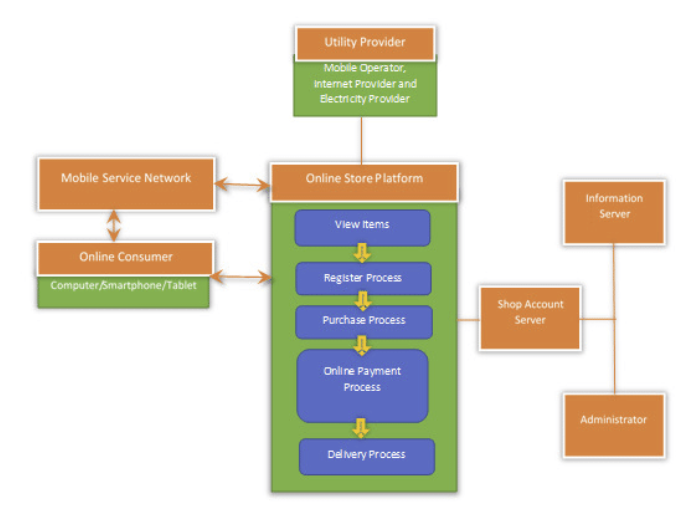
\includegraphics[width=\textwidth]{images/Architecturepattern.png}
    \caption{Architecture Pattern For Online Shopping Application}
    \label{fig:usecase3}
\end{figure}


\section{Appendix D}

\subsection{Activity Diagram}
\begin{figure}[H] % Use 'H' to place the figure exactly here
    \centering
    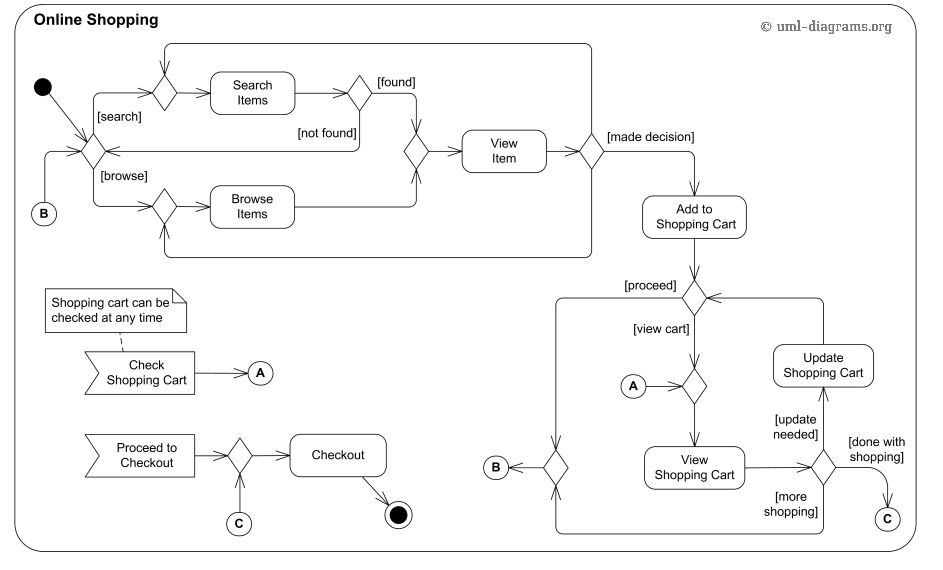
\includegraphics[width=\textwidth]{images/activityexample.png}
    \caption{Activity Diagram For Online Shopping Application}
    \label{fig:usecase3}
\end{figure}


\subsection{Class Diagram}
\begin{figure}[H] % Use 'H' to place the figure exactly here
    \centering
    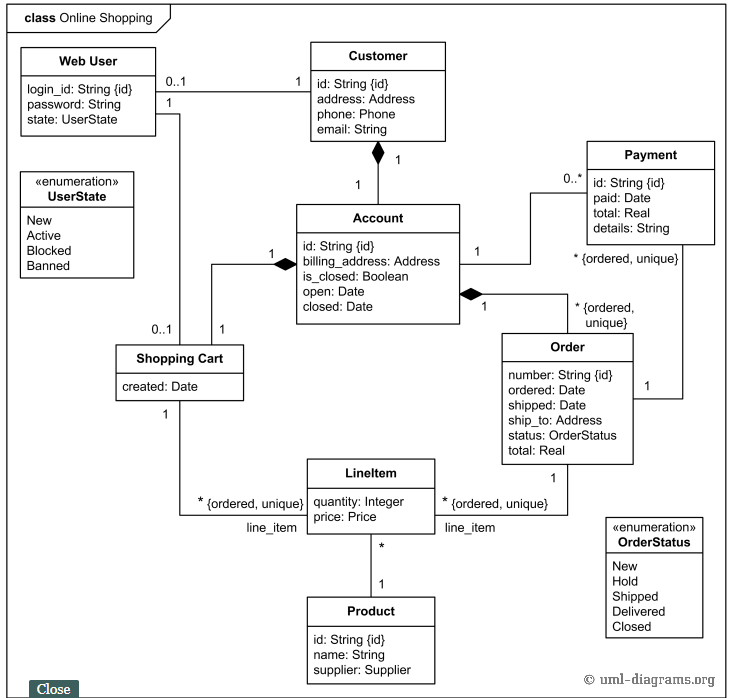
\includegraphics[width=\textwidth]{images/classexample.png}
    \caption{Class Diagram For Online Shopping Application}
    \label{fig:usecase3}
\end{figure}

\subsection{Sequence Diagram}
\begin{figure}[H] % Use 'H' to place the figure exactly here
    \centering
    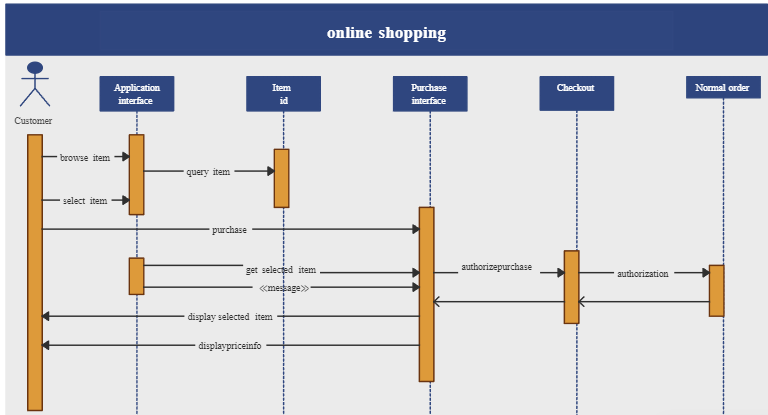
\includegraphics[width=\textwidth]{images/sequenceexample.png}
    \caption{Sequence Diagram For Online Shopping Application}
    \label{fig:usecase3}
\end{figure}

\subsection{State Transition Diagram}
\begin{figure}[H] % Use 'H' to place the figure exactly here
    \centering
    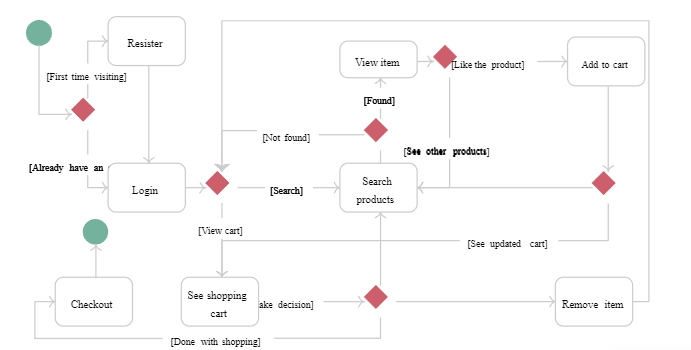
\includegraphics[width=\textwidth]{images/statetransitionexample.png}
    \caption{State Transition Diagram For Online Shopping Application}
    \label{fig:usecase3}
\end{figure}

\subsection{Data Flow Diagram}
\begin{figure}[H] % Use 'H' to place the figure exactly here
    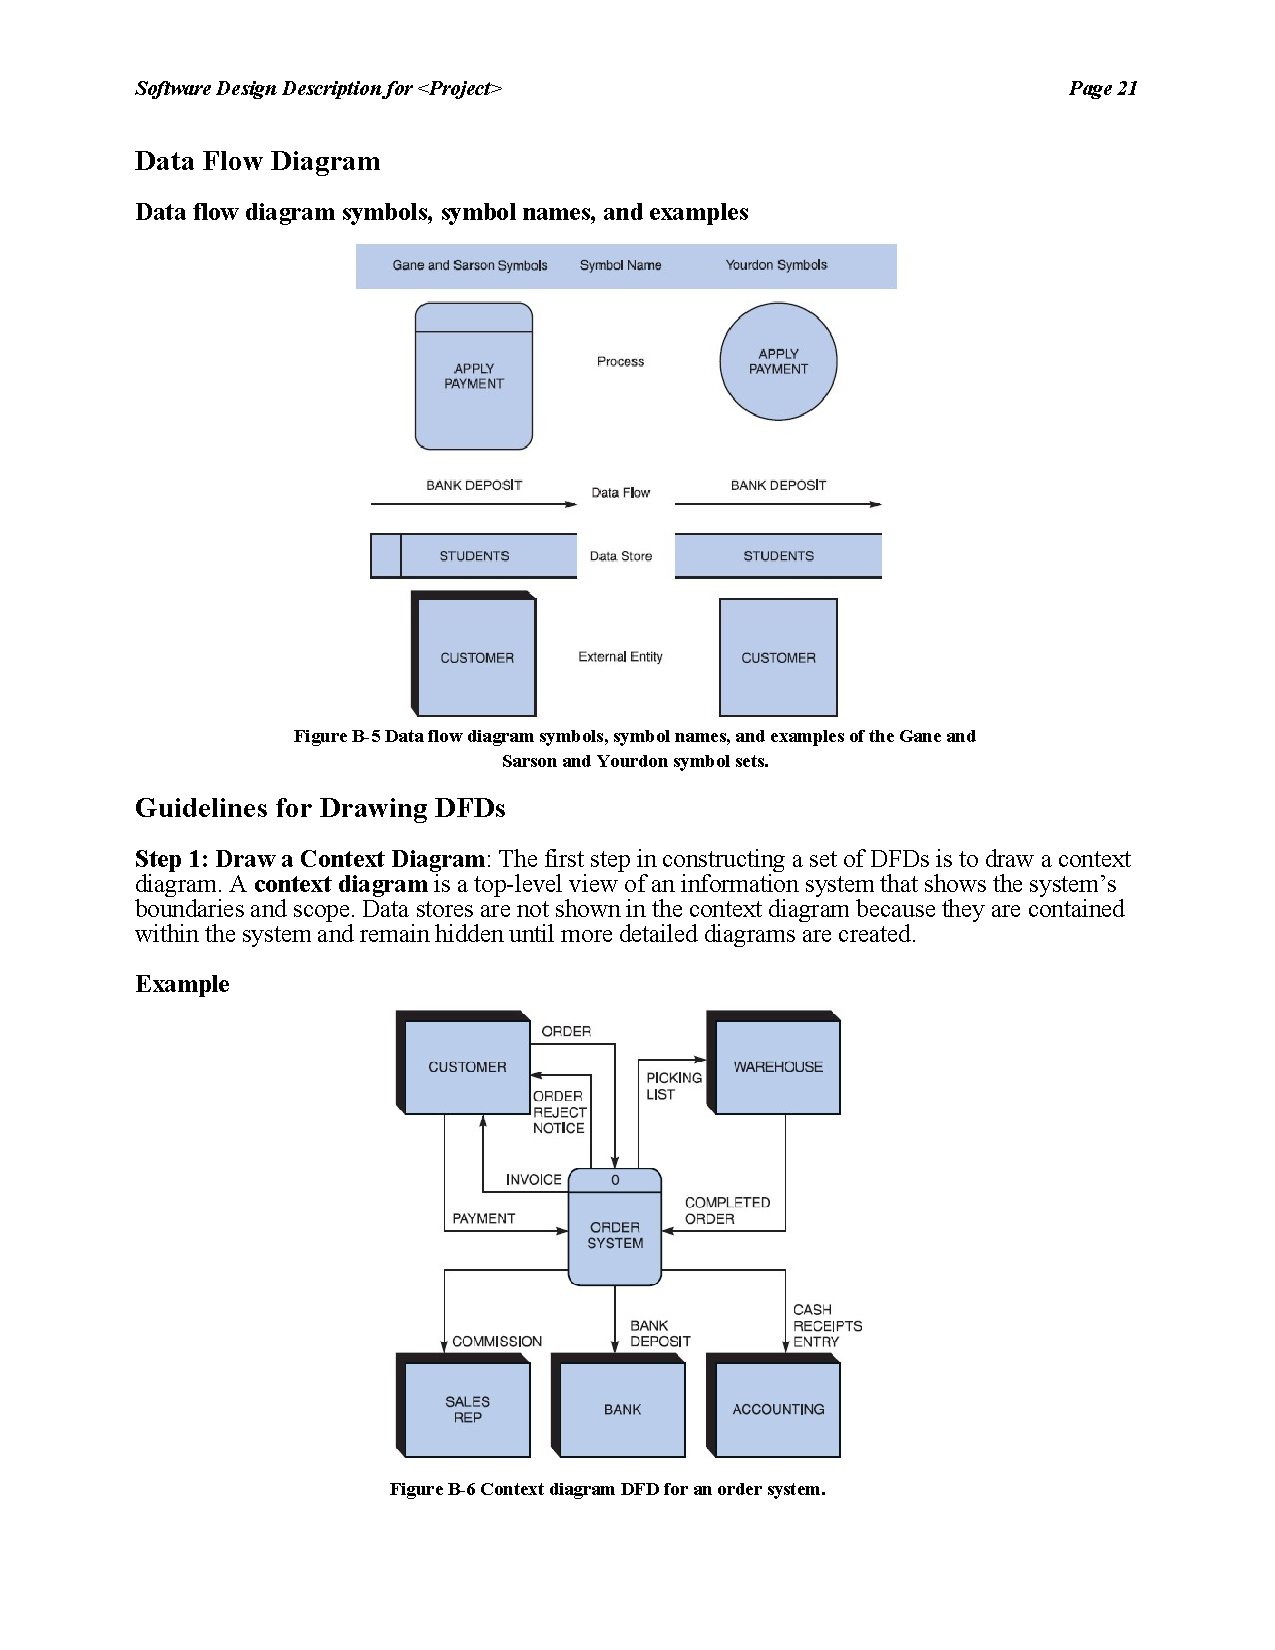
\includegraphics[scale=0.9]{DFD.pdf}
    % 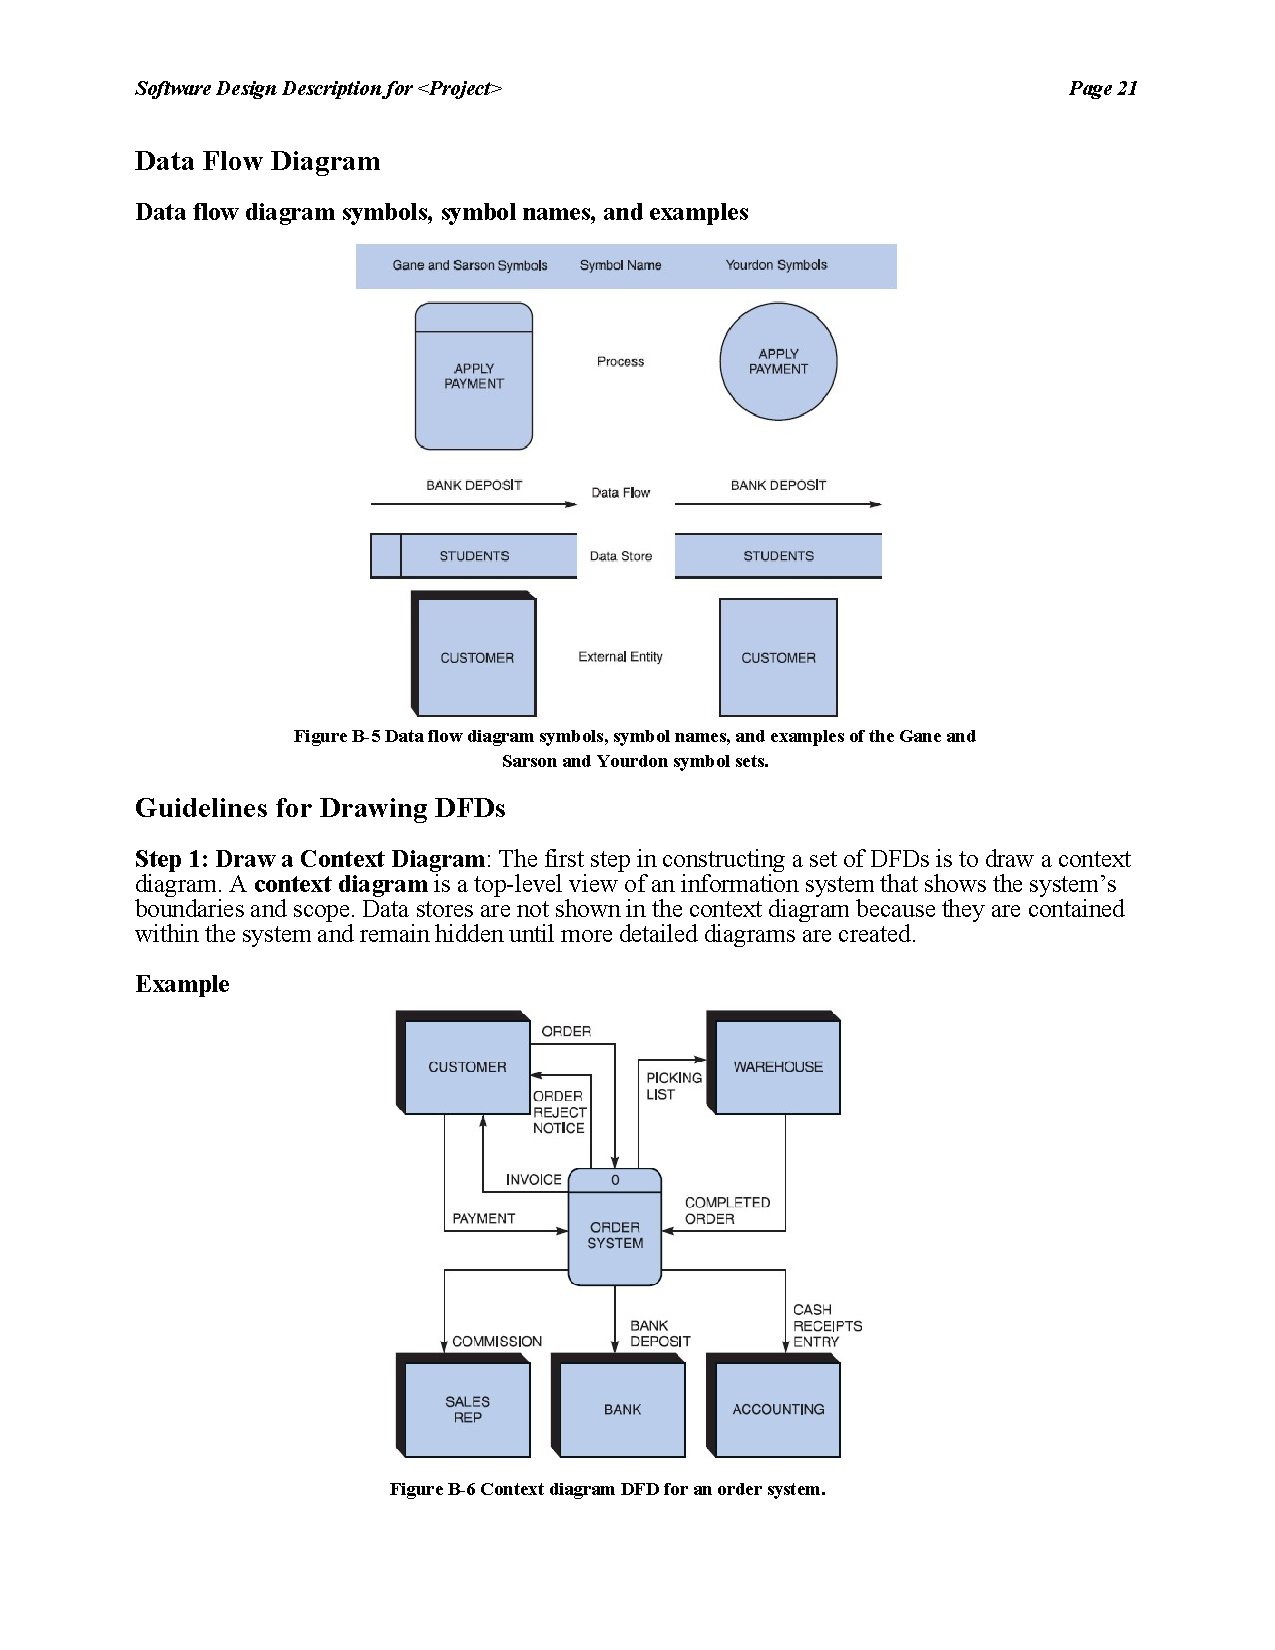
\includegraphics[width=\textwidth]{DFD.pdf}
\end{figure}
\begin{figure}[H] % Use 'H' to place the figure exactly here
    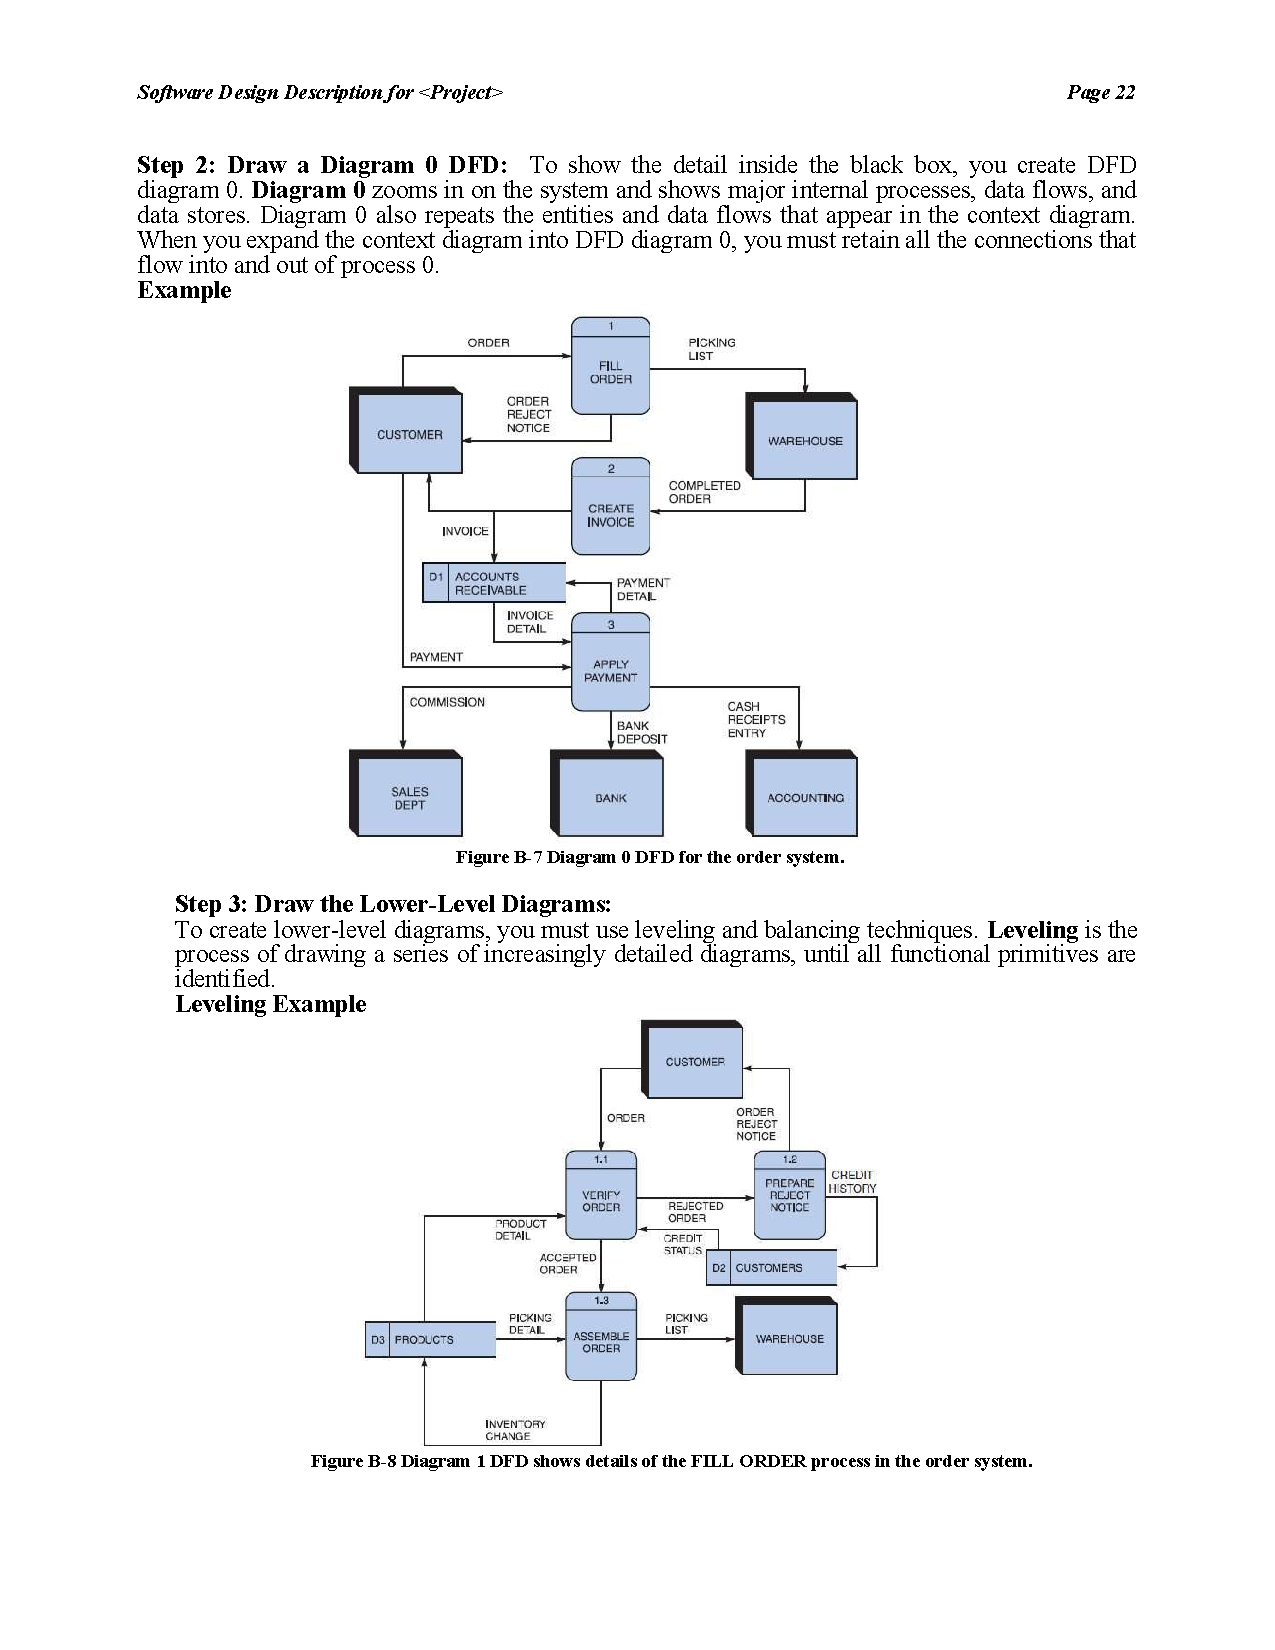
\includegraphics[scale=0.9]{DFD2.pdf}
    % 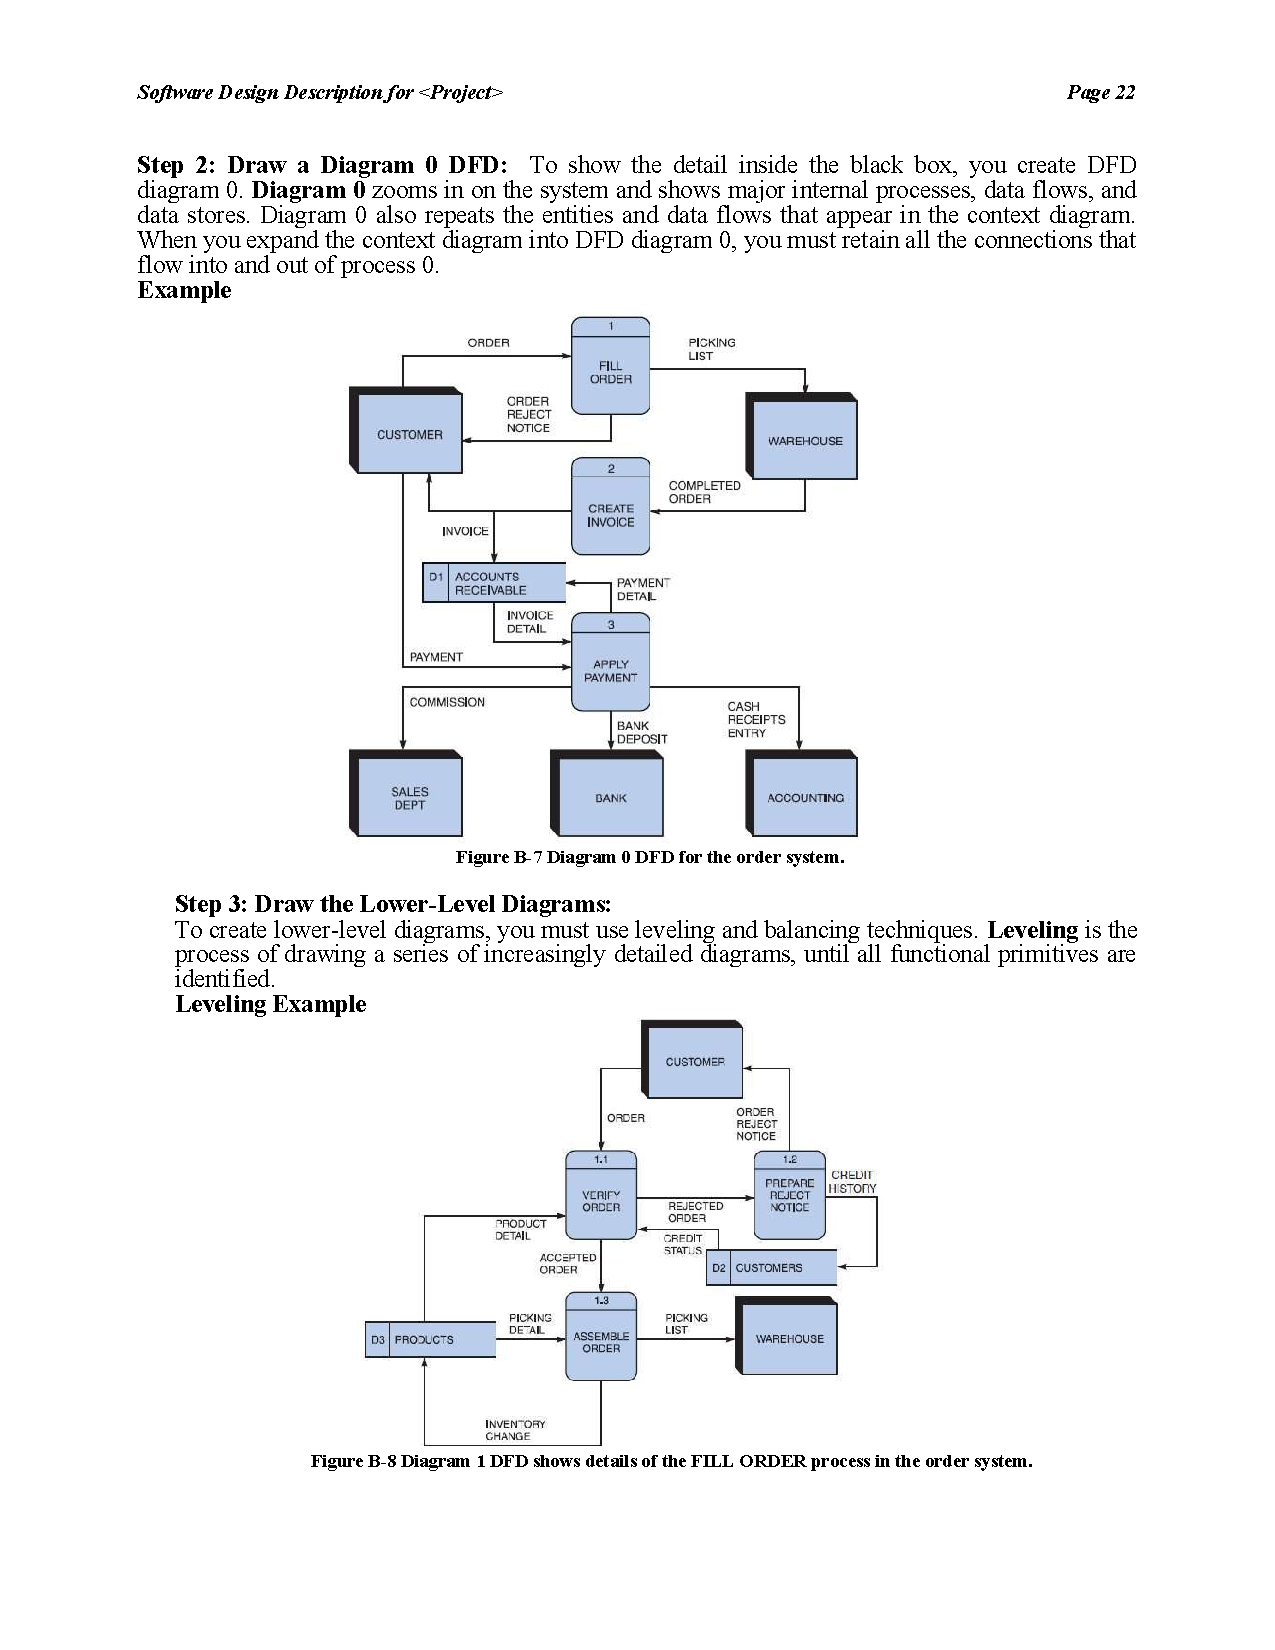
\includegraphics[width=\textwidth]{DFD2.pdf}
\end{figure}